\begin{frame}{Methodology}
    \centering
    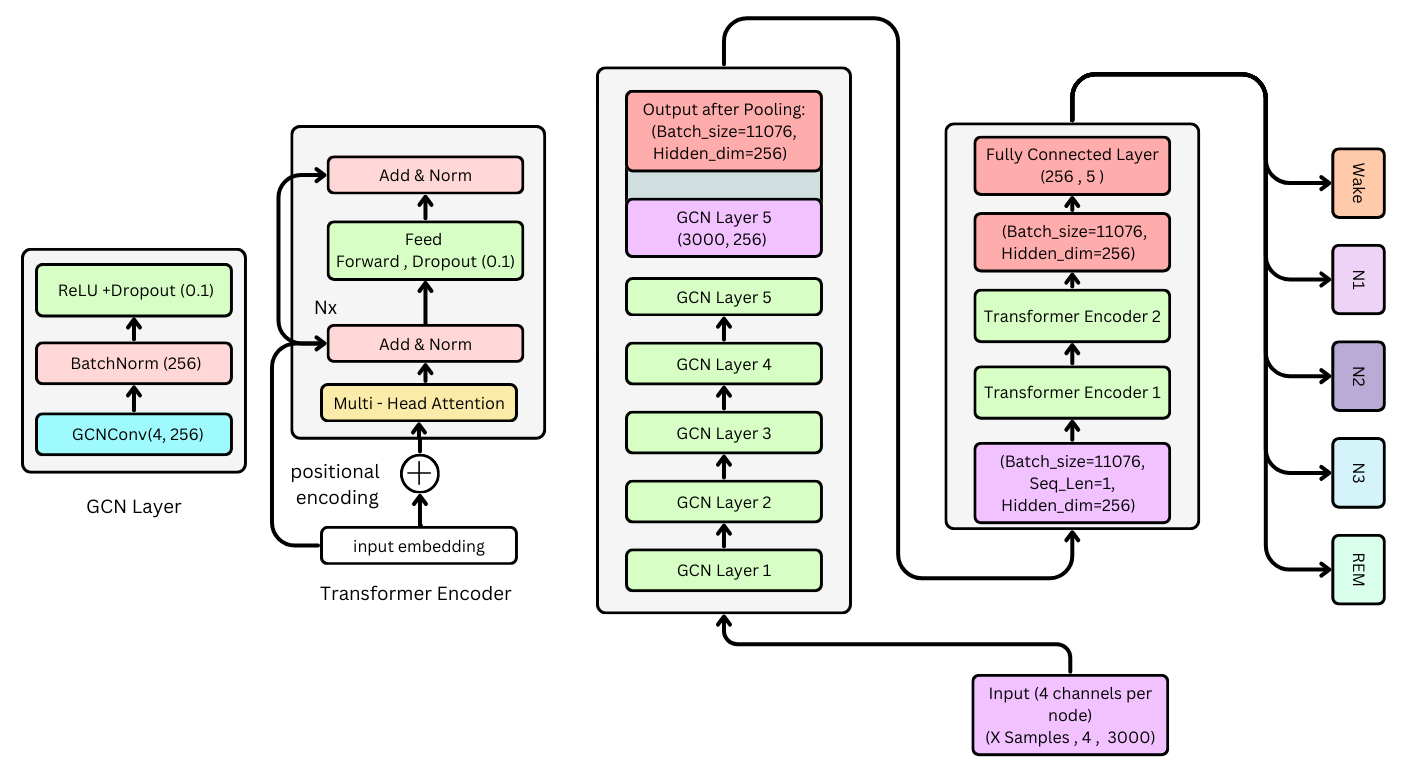
\includegraphics[width=0.85\linewidth]{figures/Architechture.png} % Slightly smaller image

        \small \textbf{Figure:} Proposed SleepGCN-Transformer Architecture % Smaller caption
\end{frame}

\begin{frame}{Methodology: Preprocessing}
    \begin{columns}
        % Left Column: Channel Selection
        \column{0.50\textwidth}
        \textbf{Channel Selection:}
        \begin{itemize}
            \item Extracting four relevant EEG channels:
            \begin{itemize}
                \item EEG Fpz-Cz
                \item EEG Pz-Oz
                \item EMG submental
                \item EOG horizontal
            \end{itemize}
        \end{itemize}

        % Right Column: Sleep Stage Mapping
        \column{0.50\textwidth}
        \textbf{Sleep Stage Mapping:}
        \begin{table}[]
            \centering
            \renewcommand{\arraystretch}{1.2}
            \begin{tabular}{|c|c|}
                \hline
                \textbf{Original Stage} & \textbf{Mapped Label} \\
                \hline
                Sleep stage W  & 0 \\
                Sleep stage 1  & 1 \\
                Sleep stage 2  & 2 \\
                Sleep stage 3  & 3 \\
                Sleep stage 4  & 3 \\
                Sleep stage R  & 4 \\
                \hline
            \end{tabular}
        \end{table}
    \end{columns}
\end{frame}









\begin{frame}{Methodology: Preprocessing}
    \textbf{Epoch Segmentation:}
    \begin{itemize}
        \item EEG signals are segmented into 30-second epochs.
        \item Each epoch contains 3000 samples per channel.
    \end{itemize}

    \vspace{10pt}
    \textbf{Band-Pass Filtering:}
    \begin{itemize}
        \item A band-pass filter (0.3 - 30 Hz) is applied.
        \item Signals above 30 Hz are removed to eliminate noise.
    \end{itemize}

    \vspace{10pt}
    \textbf{Final Data Shape:}  
    \[
    \text{[X, 4, 3000]}  
    \]

    \end{frame}


\begin{frame}{Methodology: Graph Dataset Creation}

    \begin{columns}
    
        % Left Column: Graph Adjacency Matrix
        \column{0.50\textwidth}
        \textbf{Graph Adjacency Matrix (Edge Weights):}
        \centering
        \renewcommand{\arraystretch}{1.2}
        \resizebox{\linewidth}{!}{ % Ensures table fits within the column
            \begin{tabular}{|c|c|c|c|c|}
                \hline
                & \textbf{Fpz-Cz} & \textbf{Pz-Oz} & \textbf{EMG} & \textbf{EOG} \\
                \hline
                \textbf{Fpz-Cz} & 0   & 0.9 & 0.6 & 0.6 \\
                \textbf{Pz-Oz}  & 0.9 & 0   & 0.6 & 0.6 \\
                \textbf{EMG}    & 0.6 & 0.6 & 0   & 0.5 \\
                \textbf{EOG}    & 0.6 & 0.6 & 0.5 & 0   \\
                \hline
            \end{tabular}
        }

        \vspace{8pt}

        \textbf{Dataset Information:}
        \begin{itemize}
            \item Total Samples: 11,076
            \item Example Sample Format:
        \end{itemize}

  
        \text{Data(x=[3000, 4], edge\_index=[2, 12],}
  
        \text{edge\_attr=[12], y=[1])}
      

        % Right Column: Graph Representation
        \column{0.50\textwidth}
        \centering
        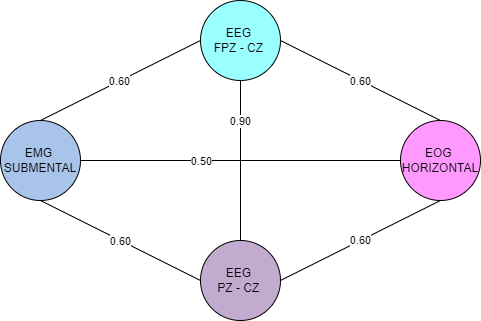
\includegraphics[width=0.85\linewidth]{figures/Graph Weightage.png} % Replace with actual graph image

        {\textcolor{purple}{\small Graph Representation of EEG Channels}}

    \end{columns}
\end{frame}



\begin{frame}{Methodology: Graph Convolutional Layer}
    \begin{columns}[c] % Align columns at the center for better layout

        % Left Column: Explanation and Data Shapes
        \column{0.50\textwidth}
        
        \textbf{Graph Convolutional Layer (GCL)}
        \vspace{5pt}
        \begin{itemize}
            \item Captures spatial relationships in EEG signals.
            \item Learns connectivity patterns between EEG channels.
            \item Enhances feature extraction by leveraging graph structures.
        \end{itemize}

        \vspace{8pt} % Adjust spacing for better layout
        \textbf{Tensor Shapes for GCL Input:}
        \vspace{3pt}
        \begin{itemize}
            \item \textbf{X\_all}: (11076, 4, 3000)
            \item \textbf{Y\_all}: (11076,)
            \item \textbf{X\_tensor}: \texttt{torch.Size([11076, 4, 3000])}
            \item \textbf{Y\_tensor}: \texttt{torch.Size([11076])}
            \item \textbf{Sample x}: \texttt{torch.Size([3000, 4])}
            \item \textbf{Sample edge\_index}: \texttt{torch.Size([2, 12])}
            \item \textbf{Sample y}: \texttt{torch.Size([1])}
        \end{itemize}

        % Right Column: GCL Image with Proper Caption
        \column{0.50\textwidth}
        \centering
        \vspace{-10pt} % Adjust vertical spacing for better fit
        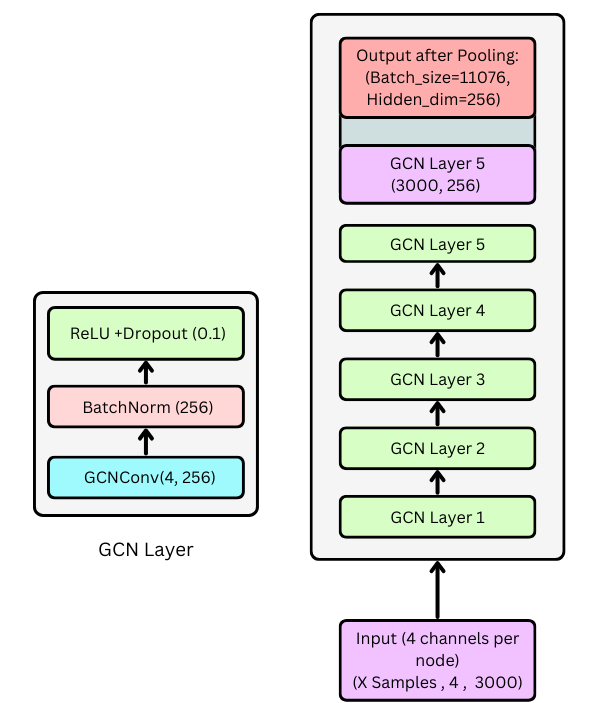
\includegraphics[width=0.6\linewidth]{figures/Graph Convolution Neural Network.png} % Adjusted path and width

        % Proper caption placement
        \vspace{0.3cm}
        \small{\textcolor{uwopurple}{Graph Convolutional Layer Representation}}

    \end{columns}
\end{frame}


\begin{frame}{Methodology: GCN Tensor Details and Global Pooling}
    \centering % Center the entire content for better alignment

    \textbf{Additional Tensor Shapes for GCL:}
    \vspace{5pt} % Adjust spacing for better readability
    \begin{itemize}
        \item \textbf{Sample x}: \texttt{torch.Size([3000, 4])}
        \item \textbf{Sample edge\_index}: \texttt{torch.Size([2, 12])}
        \item \textbf{Sample y}: \texttt{torch.Size([1])}
    \end{itemize}

    \vspace{10pt} % Space between sections
    \textbf{Global Mean Pooling:}
    \vspace{5pt}
    \begin{itemize}
        \item \textbf{Input:} Node embeddings from GCN layers (e.g., (3000, 256))
        \item \textbf{Operation:} Mean pooling over nodes based on batch indices
        \item \textbf{Output:} Graph-level embedding (e.g., (Batch\_size=11076, 256))
    \end{itemize}

\end{frame}



\begin{frame}{Methodology: Transformer Encoder}
    \begin{columns}

        % Left Column: Details
        \column{0.50\textwidth}

        \textbf{\large Transformer Encoder Overview}
        \vspace{5pt}
        \begin{itemize}
            \item \textbf{Preprocessing:} Expand graph embedding to \texttt{(Batch, 1, 256)}
            \item \textbf{Transformer Encoder:} 
            \begin{itemize}
                \item \textbf{2 Transformer Encoder Layers} with:
                \begin{itemize}
                    \item \textbf{d\_model = 256}
                    \item \textbf{nhead = 4}
                    \item \textbf{dropout = 0.1}
                    \item \texttt{batch\_first=True}
                \end{itemize}
            \end{itemize}
            \item \textbf{Postprocessing:} Squeeze output to \texttt{(Batch, 256)}
        \end{itemize}

        \vspace{10pt}
        \textbf{\large Fully Connected Layer}
        \vspace{5pt}
        \begin{itemize}
            \item \textbf{Linear Layer:} \texttt{Linear(256 → 5)}
            \item \textbf{Output:} Logits for 5-class classification
        \end{itemize}

        % Right Column: Transformer Figure
        \column{0.50\textwidth}
        \centering
        % \vspace{-}
        \includegraphics[width=\linewidth]{figures/Transformer.png} % Replace with actual image
        \vspace{2pt}
        \captionof{figure}{\textcolor{uwopurple}{Transformer Encoder Architecture}}

    \end{columns}
\end{frame}

\begin{frame}{Methodology: Why Focal Loss Instead of Standard Cross-Entropy?}

    \textbf{\large Motivation for Focal Loss}
    \vspace{5pt}
    \begin{itemize}
        \item Standard Cross-Entropy treats all samples equally, leading to bias towards majority classes.
        \item In imbalanced datasets, minority class predictions get suppressed.
        \item \textbf{Focal Loss} dynamically adjusts loss contribution based on prediction confidence.
        \item It reduces the importance of well-classified samples and focuses more on hard-to-classify ones.
    \end{itemize}

    \vspace{10pt}
    \textbf{\large Key Features of Focal Loss}
    \vspace{5pt}
    \begin{itemize}
        \item Introduces a focusing parameter \( \gamma \) to adjust class weighting.
        \item Includes class weighting factor \( \alpha \) to handle imbalance.
        \item Works well for highly imbalanced datasets in classification tasks.
    \end{itemize}

\end{frame}
\begin{frame}{Methodology: Focal Loss Formulation}

    \textbf{\large Mathematical Formulation}
    \vspace{5pt}

    \[
    \text{FL}(p_t) = -\alpha (1 - p_t)^{\gamma} \log(p_t)
    \]

    where:
    \begin{itemize}
        \item \( p_t \) is the predicted probability for the target class.
        \item \( \alpha \) is the weighting factor for class imbalance.
        \item \( \gamma \) is the focusing parameter (higher values focus more on hard examples).
    \end{itemize}

    \vspace{10pt}
    \textbf{\large Implementation Details}
    \vspace{5pt}
    \begin{itemize}
        \item Label smoothing:  
              \[
              y_{\text{smooth}} = y(1 - \epsilon) + \frac{\epsilon}{C}
              \]
        \item Prevents log(0) issue by adding a small constant \( \epsilon \).
        \item PyTorch-based computation:  
              \[
              \mathcal{L} = \alpha (1 - p)^{\gamma} (-y_{\text{smooth}} \log p)
              \]
    \end{itemize}

\end{frame}


\begin{frame}{Why Use a Learning Rate Scheduler?}

    \textbf{\large Importance of Learning Rate Scheduling}
    \vspace{5pt}
    \begin{itemize}
        \item The learning rate is crucial for training deep models efficiently.
        \item A high learning rate can lead to divergence, while a low one may cause slow convergence.
        \item Adaptive learning rate schedules help balance stability and speed.
    \end{itemize}

    \vspace{10pt}
    \textbf{\large Why CosineAnnealingLR?}
    \vspace{5pt}
    \begin{itemize}
        \item Smoothly reduces the learning rate following a cosine decay.
        \item Starts with a large step size for exploration and gradually fine-tunes.
        \item Helps avoid sharp drops in the learning rate, improving generalization.
    \end{itemize}

\end{frame}



\begin{frame}{Cosine Annealing Learning Rate Decay}

    \textbf{\large Cosine Annealing Formula:}
    \[
    \eta_t = \eta_{\text{min}} + \frac{1}{2} (\eta_{\text{max}} - \eta_{\text{min}}) 
    \left( 1 + \cos \left( \frac{T_{cur}}{T_{max}} \pi \right) \right)
    \]
    where:
    \begin{itemize}
        \item \( \eta_t \) is the learning rate at epoch \( t \).
        \item \( \eta_{\text{max}} \) and \( \eta_{\text{min}} \) are the max/min learning rates.
        \item \( T_{cur} \) is the current epoch.
        \item \( T_{max} \) is the total number of epochs.
    \end{itemize}

    \vspace{10pt}
    \textbf{\large Key Benefits:}
    \begin{itemize}
        \item Encourages large updates early in training.
        \item Smoothly transitions into finer updates as training progresses.
        \item Helps the model avoid getting stuck in poor local minima.
    \end{itemize}

\end{frame}


\begin{frame}{Training Methodology: Overview}

    \textbf{\large SleepTrainer Class: Key Features}
    \vspace{5pt}
    \begin{itemize}
        \item Handles model training, validation, and optimization.
        \item Uses \textbf{Focal Loss} to address class imbalance.
        \item Applies \textbf{CosineAnnealingLR} scheduler for smooth learning rate decay.
    \end{itemize}

    \vspace{10pt}
    \textbf{\large Training Process}
    \vspace{5pt}
    \begin{enumerate}
        \item Compute class weights for imbalanced data.
        \item Iterate through training batches, compute loss and update weights.
        \item Validate model performance on a separate validation set.
        \item Adjust learning rate dynamically using a scheduler.
    \end{enumerate}

\end{frame}


\begin{frame}{Training Methodology: Hyperparameters}

    \textbf{\large Key Hyperparameters}
    \vspace{5pt}
    \begin{itemize}
        \item \textbf{Batch Size:} 32  \hfill 
        \item \textbf{Learning Rate:} 0.0003  \hfill
        \item \textbf{Weight Decay:} \( 1e^{-4} \)  \hfill 
        \item \textbf{Epochs:} 20  \hfill 
        \item \textbf{Optimizer:} AdamW  \hfill 
    \end{itemize}

    \vspace{10pt}
    \textbf{\large Learning Rate Scheduler: CosineAnnealingLR}
    \begin{itemize}
        \item Gradually reduces learning rate over time for smooth convergence.
        \item Helps prevent sudden drops in performance.
    \end{itemize}

\end{frame}

\begin{frame}{Training Methodology: Handling Class Imbalance}

    \textbf{\large Why Compute Class Weights?}
    \vspace{5pt}
    \begin{itemize}
        \item EEG sleep data is imbalanced, with some sleep stages appearing more frequently.
        \item Without weighting, the model may favor majority classes.
        \item Weights ensure rare classes contribute more to the loss.
    \end{itemize}

    \vspace{10pt}
    \textbf{\large Class Weight Computation}
    \vspace{5pt}
    \[
    w_c = \left( \frac{\text{Total Samples}}{\text{Class Count} + 1} \right)^{0.5}
    \]
    where:
    \begin{itemize}
        \item \( w_c \) is the computed weight for class \( c \).
        \item Small classes receive higher weights.
        \item Weights are applied to Focal Loss for training.
    \end{itemize}

\end{frame}




 